
\begin{defn}[Independent Events]\index{independent events}
    When one action does not influence the outcome of another action, such as rolling two different dice, we say they are \emph{independent events}.
\end{defn}

\begin{defn}[Disjoint Events]\index{disjoint events}
    When two outcomes can not happen at the same time, such as a number being both even and odd, we say that they are \emph{disjoint events}.
\end{defn}

\begin{defn}[Multiplication Principle]\index{multiplication principle}
    If we have \(k\) \emph{independent} choices to make and \(n_i\) options for each choice, then the total number of possible choices is
        \[\prod_{i=1}^kn_i=n_1\times n_2\times\cdots\times n_k.\]
\end{defn}

\begin{defn}[Addition Principle]\index{addition principle}
    If we have \(k\) \emph{disjoint} options and each option can be chosen in \(n_i\) different ways, then the total number of options is
        \[\sum_{i=1}^{k}n_i=n_1+n_2+\cdots+n_k.\]
\end{defn}

\clearpage

\begin{exposition}
    As you enter Sandwich-Way you see the following directions for making a sandwich:
    \begin{enumerate}
        \item Choose one of 12 bread options.
        \item Choose one of 16 ``Protein'' options.
        \item Choose up to 1 of 7 cheese options.
        \item Choose up to 3 of 10 vegetable options.
        \item Choose up to 3 of 13 condiments.
    \end{enumerate}
    You then find yourself wondering how many different sandwiches you can make.

    \noindent%
    What are the number of sandwiches if we use the \emph{minimum} number of ingredients?
    \begin{align*}
        Bread\times Protein\times Cheese\times Vegetables\times &Condiments\\
            &= 12\times 16\times 1\times 1\times 1\\
            &= 192\ Sandwiches
    \end{align*}

    \noindent%
    What are the number of sandwiches if we use the \emph{maximum} number of ingredients (without repetition)?\footnote{For simplicity we are assuming we care what order cheeses and condiments are added.}
    \begin{align*}
        Bread\times Protein\times Cheese\times Vegetables\times &Condiments\\
            &= 12\times 16\times 7\times (10\cdot9\cdot8)\times (13\cdot12\cdot11)\\
            &= 1,660,538,880\ Sandwiches
    \end{align*}

    \noindent%
    How many sandwiches are there if we either minimize or maximize the number of ingredients?
    \[192\ Sandwiches+1,660,538,880\ Sandwiches=1,660,539,072\ Sandwiches\]
\end{exposition}


\begin{practiceprob}{Returning for Another Sandwich}
    How many different sandwiches are there with no vegetables?\vspace{0.1\textheight}

    What if you really like dry sandwiches with no condiments?\vspace{0.1\textheight}

\end{practiceprob}


\begin{exposition}\index{decision tree}
We can map out and compile a sequence of options using a \emph{decision tree}.  For example here is how we can create a sandwich with one or no choice of protein and one or no choice of cheese.
\begin{figure}[H]
    \centering
    % \inputtikz{decision_tree}
    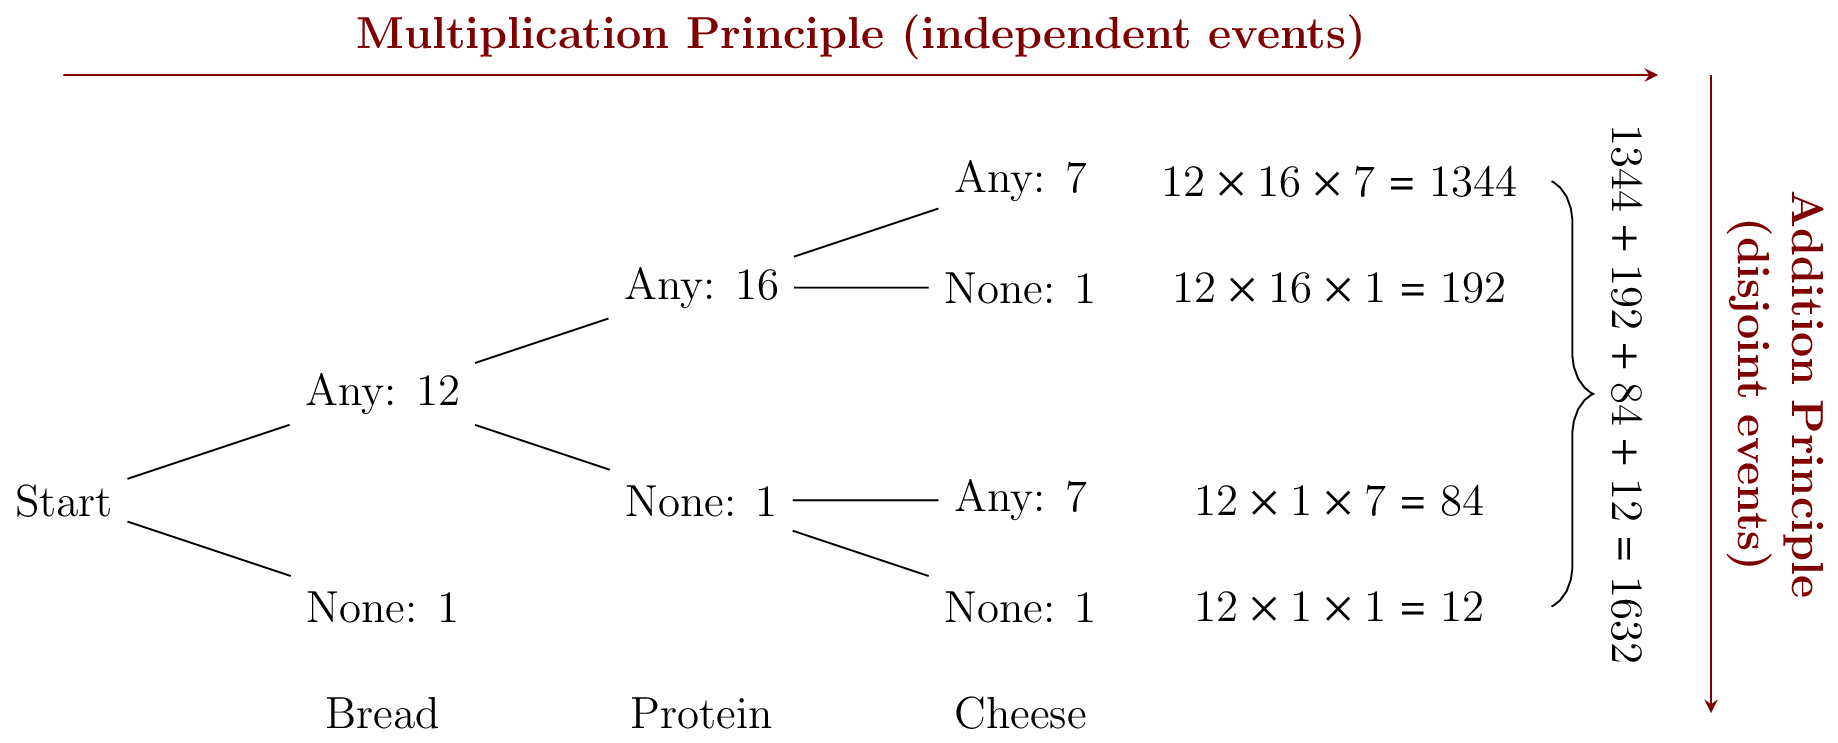
\includegraphics[scale=0.24,alt={decision tree used to coutn the ways to make a sandwich}]{images/created/decision_tree.png}
    \caption{Sandwich Decision Tree}
    \label{fig:sandwich-tree}
\end{figure}
Note that for small examples/simple situations we can actually draw a decision tree, for anything particularly large it is a useful organizational tool but not practical to draw.
\end{exposition}

\begin{practiceprob}{License Plates}
    Suppose that all the license plates in a state must consist of a digit from 1 to 9, followed by four different letters, followed by a different digit from 1-9. How many different license plates could we create? What if you could repeat letters or numbers? What if you could also choose two of four colors?
    \begin{center}
        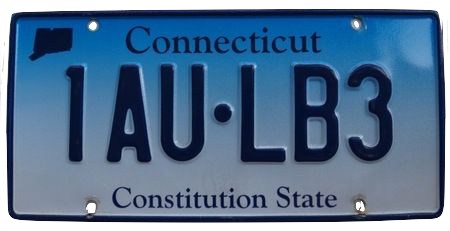
\includegraphics[width=2in,alt={license plate with a number four letters and a number}]{images/LicensePlate.png}
    \end{center}
    \vspace{0.25\textheight}
\end{practiceprob}

\clearpage

\begin{practiceprob}
    Preparing for a party you go to the store to get soda, chips, and cookies. For cookies and soda there are regular and sugar free varieties, and for chips there is regular or low sodium.
    \begin{center}
        \begin{tabular}{|*{7}{m{0.115\textwidth}}|}\hline
            &\multicolumn{2}{c}{Soda}
            &\multicolumn{2}{c}{Chips}
            &\multicolumn{2}{c|}{Cookies} \tabularnewline
             & Regular & Sugar Free 
             & Regular & Low Salt
             & Regular & Sugar Free \tabularnewline
             Varieties & 10 & 7 & 15 & 12 & 14 & 8 \tabularnewline \hline
        \end{tabular}
    \end{center}
    How many buying options do you have if you just get one type of each product? (Use a decision tree.)
    \vspace{0.25\textheight}
\end{practiceprob}

\begin{defn}[Inclusion-Exclusion Principle]\index{cardinality}\index{inclusion-exclusion principle}
    For any set \(X\) let \(|X|\) be the \emph{cardinality}, or size, of \(X\). Given sets \(A\), \(B\), and \(C\),
        \[|A\cup B|=|A|+|B|-|A\cap B|\]
    and \[|A\cup B\cup C|=|A|+|B|+|C|-|A\cap B|-|A\cap C|-|B\cap C|+|A\cap B\cap C|.\]
    \begin{figure}[H]
        \centering
        % \inputtikz{inclusion_exclusion}
        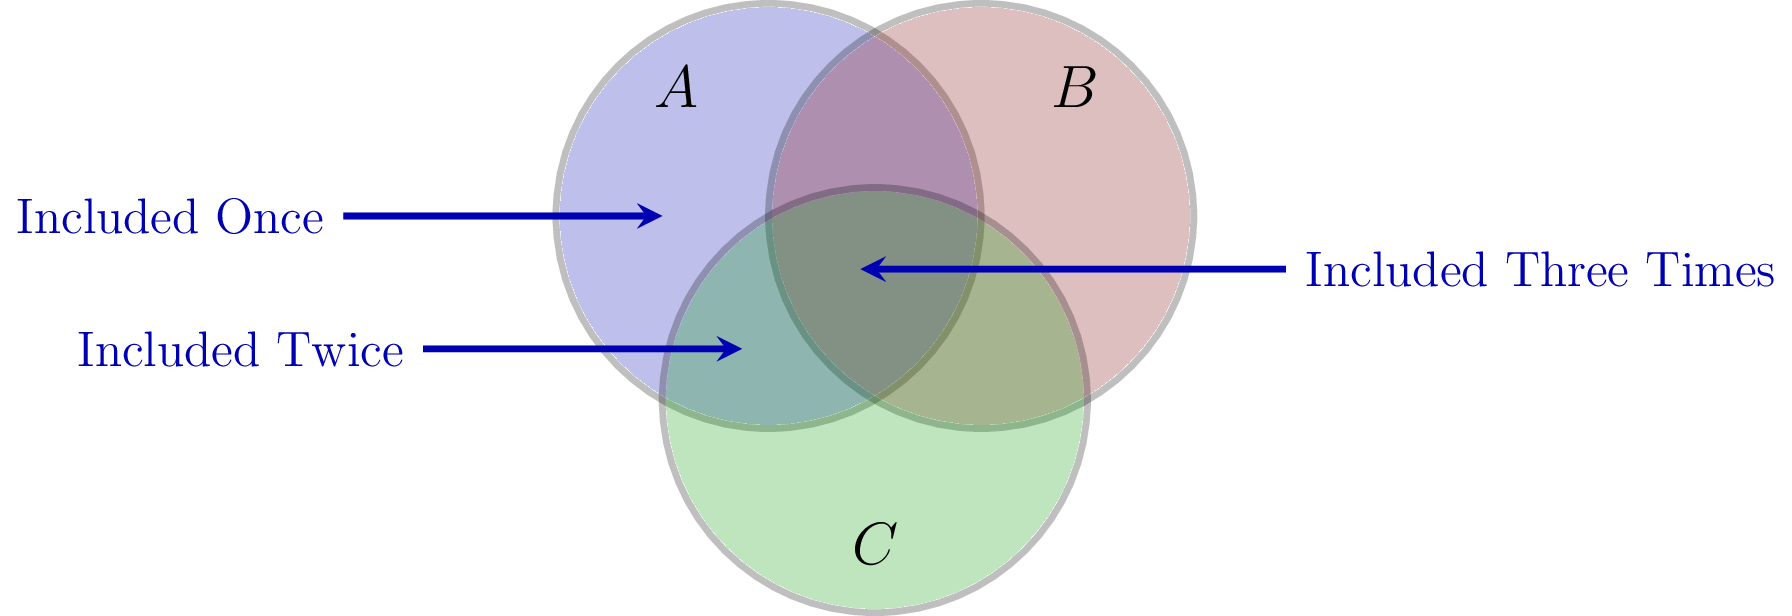
\includegraphics[scale=0.24,alt={venn diagram demonstrating the inclusion exclusion principle for three sets}]{images/created/inclusion_exclusion.png}
        \caption{Inclusion-Exclusion Principle for Three Sets}
        \label{fig:Inclusion-Exclusion}
    \end{figure}
\end{defn}

\begin{exposition}
    Let \(\overline{C}\) be the set of all sandwiches with no cheese and \(\overline{V}\) be the set of all sandwiches with no vegetables. How many sandwiches have no cheese or no vegetables?
    \begin{itemize}
        \item \(\overline{C}\) is sandwiches with no cheese.
        \item \(\overline{V}\) is sandwiches with no vegetables.
        \item \(\overline{C}\cup\overline{V}\) is sandwiches with no cheese \emph{OR} no vegetables.
        \item \(\overline{C}\cap\overline{V}\) is sandwiches with no cheese \emph{AND} no vegetables. 
    \end{itemize}
    \begin{figure}[H]
        \centering
        % \inputtikz{two_set_venn_diagram}
        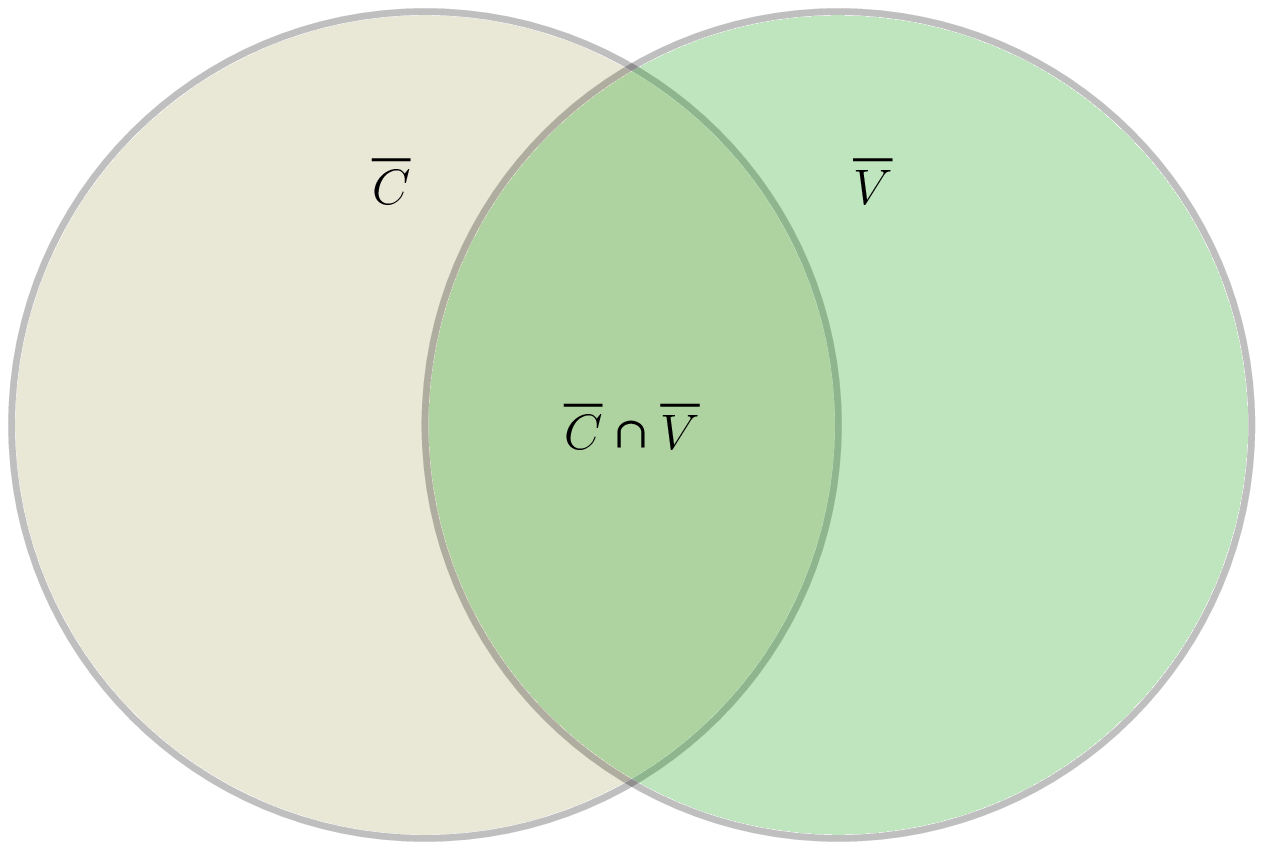
\includegraphics[scale=0.24,alt={blank venn diagram with sets for no cheese and no vegetable sandwiches}]{images/created/two_set_venn_diagram.png}
        \caption{No Cheese and/or No Vegetables}
        \label{fig:Chese_Vege_Diagram}
    \end{figure}
    Using the multiplication and addition principles we can get:
    \begin{align*}
        |\overline{C}|&= 12,773,376\\
        |\overline{V}|&= 580,608\\
        |\overline{C}\cap\overline{V}|&=72,576
    \end{align*}
    Therefore, the number of sandwiches with no cheese or no vegetables is:
    \begin{align*}
        |\overline{C}\cup\overline{V}|&=|\overline{C}|+|\overline{V}|-|\overline{C}\cap\overline{V}|\\
            &=12773376+580608-75576\\
            &=13,278,408
    \end{align*}
\end{exposition}

\clearpage

\begin{practiceprob}
    Your license plates consisting of a digit from 1 to 9, followed by four different letters, followed by a different digit from 1-9, have been getting complaints because people confuse the B with the 8.  To solve this problem you need to exclude one of both of these characters, in how many ways can you do that?
    \vspace{0.3\textheight}
\end{practiceprob}

\begin{practiceprob}
    Suppose you need to get sugar free soda or sugar free cookies, in how many ways could you do that?
    \begin{center}
        \begin{tabular}{|*{7}{m{0.115\textwidth}}|}\hline
            &\multicolumn{2}{c}{Soda}
            &\multicolumn{2}{c}{Chips}
            &\multicolumn{2}{c|}{Cookies} \tabularnewline
             & Regular & Sugar Free 
             & Regular & Low Salt
             & Regular & Sugar Free \tabularnewline
             Varieties & 10 & 7 & 15 & 12 & 14 & 8 \tabularnewline \hline
        \end{tabular}
    \end{center}
    \vspace{0.3\textheight}
\end{practiceprob}